\documentclass{beamer}
\usetheme{Warsaw}
\usefonttheme{serif}

%My Stuff
\newcommand{\set}[1]{ \left\{ #1 \right\} }
\newcommand{\abs}[1]{\left | {#1} \right |}
\newcommand{\floor}[1]{\left \lfloor{#1} \right \rfloor}
\newcommand{\ceil}[1]{\left \lceil{#1} \right \rceil}
\newcommand{\paren}[1]{\left ({#1} \right )}
\newcommand{\brac}[1]{\left [{#1} \right ]}
\newcommand{\abrac}[1]{\left \langle{ #1} \right \rangle}
\newcommand{\norm}[1]{\left \|{#1} \right \|}
\newcommand{\CC}{\mathbb{C}}
\newcommand{\RR}{\mathbb{R}}
\newcommand{\QQ}{\mathbb{Q}}
\newcommand{\ZZ}{\mathbb{Z}}
\newcommand{\NN}{\mathbb{N}}
\newcommand{\FF}{\mathbb{F}}
\newcommand{\eps}{\varepsilon}
\newcommand{\Hh}{\mathcal{H}}
\newcommand{\Ww}{\mathcal{W}}
\newcommand{\Jj}{\mathcal{J}}
\newcommand{\Kk}{\mathcal{K}}
\newcommand{\Ff}{\mathcal{F}}
\newcommand{\Tt}{\mathcal{T}}
\newcommand{\del}{\partial}
\newcommand{\vect}{\text{vec}}
\newcommand{\cconv}{\circledast}
\newcommand{\kron}{\otimes}
\newcommand{\Del}{\nabla}
\newcommand{\Span}{\text{span}}
\newcommand{\Sin}[1]{\;\text{sin}\!\left ({ #1} \right )}
\newcommand{\Cos}[1]{\;\text{cos}\!\left ({ #1} \right )}
\renewcommand{\i}{\mathbi{i}}
\renewcommand{\lim}{\mathop{\mathrm{limit}}}
\usepackage{hyperref}

\title{Part of Speech Tagging with HMMs}
\author{Abraham Nassar}
\date{December 13, 2016}

\begin{document}
\frame{\titlepage}


\section{Viterbi}
\subsection{Motivation}
%================================================================================%
%                                   THE PROBLEM                                  %
%================================================================================%
\frame{\frametitle{The Problem}
  Our goal is to take a sentence and find the tag sequence that maximizes probabilities. 
  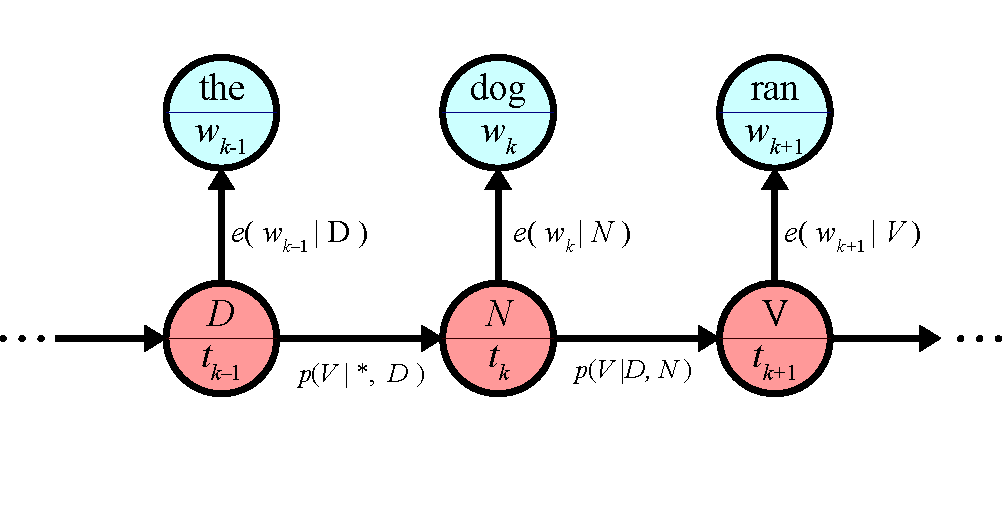
\includegraphics[width=\textwidth]{images/diagram} 
}

% Brute Force Diagram
\frame{\frametitle{The Problem}
{\bf Brute Force}: Each tag would be checked for each word. \\
\hspace{2.5cm} The number of calculations: $\paren{\#\text{tags}}^{\#\text{words}}$
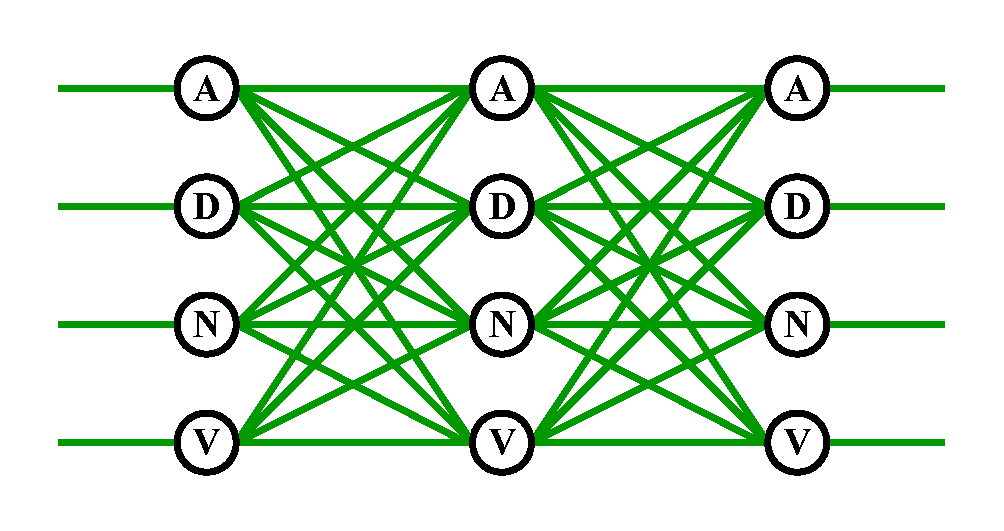
\includegraphics[width=\textwidth]{images/bruteForce}

\vspace{-0.5cm}
\hspace{1.6cm}``The" \hspace{2cm} ``dog" \hspace{2cm} ``ran" 
}

\frame{\frametitle{Definitions}
\begin{itemize}
  \item Let $\Ww$ be the set of words
  \item Let $\Tt$ be the set of tags union with $\set{END}$.
  \item Let $S(k,u,v)$ the set of all tags of length $k$ such that $y_{k-1}=u$, $y_k=v$.
  \item For index  $k\in\set{1,2,\dots,n}$ and tags $u,v$ we can define
  \[
    \pi(k,u,v) = \max_{\set{y_i}\in S(k,u,v)} \prod_{i=1}^k q(y_i|y_{i-2},y_{i-1}) \prod_{i=1}^k e(x_i|y_i)
  \]
\end{itemize}

}

\subsection{The Algorithm }
%================================================================================%
%                                  THE ALGORITHM                                 %
%================================================================================%
\frame{\frametitle{The Basic Viterbi Algorithm}

{\bf Input}: A sentence $w_1, w_2, \dots, w_n$, transition probabilities $q(t_k|t_i,t_j)$ emission probabilities, $e(w_j|t_j)$
\\
{\bf Initialization}: $\pi(0|*,*)=1$ and $\pi(0|u,v)=0$,\; $\forall u,v\in\Tt$ where $u\neq*$ or $v \neq *$
\\
{\bf Algorithm}:
\begin{itemize}
  \item for $k = 1, 2, \dots, n$
    \begin{itemize}
      \item for $(u,v)\in\Tt\times\Tt$,
        \[ 
          \pi(k,u,v) = \max_{t\in\Tt}\big[
                       \pi(k-1,t,u)\cdot q(v|t,u) \cdot e(w_k|v)
                       \big]
        \]
    \end{itemize}
    \item {\bf Return}: \\
      $$\max_{u\in\Tt,v\in\Tt}\big[\pi(n,u,v)\cdot q(END|u,v)\big]$$
\end{itemize}
\pause
\vspace{2mm}
{\bf NOTE}: This returns maximum probability, but we want argmax. So keep track of indices.
}


\frame{\frametitle{Viterbi Visualized}
{\bf Viterbi}: Find the highest probability word by word.\\
\hspace{1.55cm} The number of calculations: $(\# words)\paren{\# tags}^{3}$

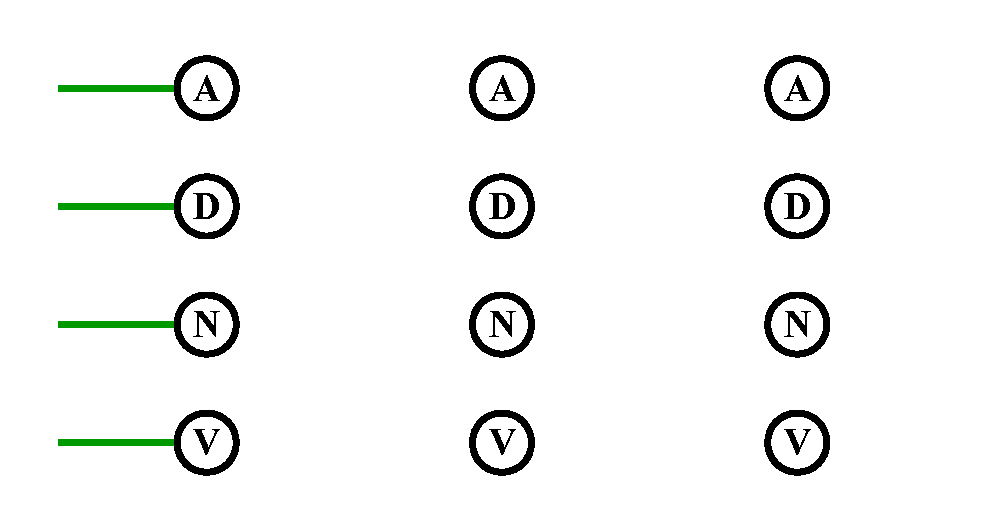
\includegraphics[width=\textwidth]{images/viterbi1}

\vspace{-0.5cm}
\hspace{1.6cm}``The" \hspace{2cm} ``dog" \hspace{2cm} ``ran" 
}
\frame{\frametitle{Viterbi Visualized}
{\bf Viterbi}: Find the highest probability word by word.\\
\hspace{1.55cm} The number of calculations: $(\# words)\paren{\# tags}^{3}$

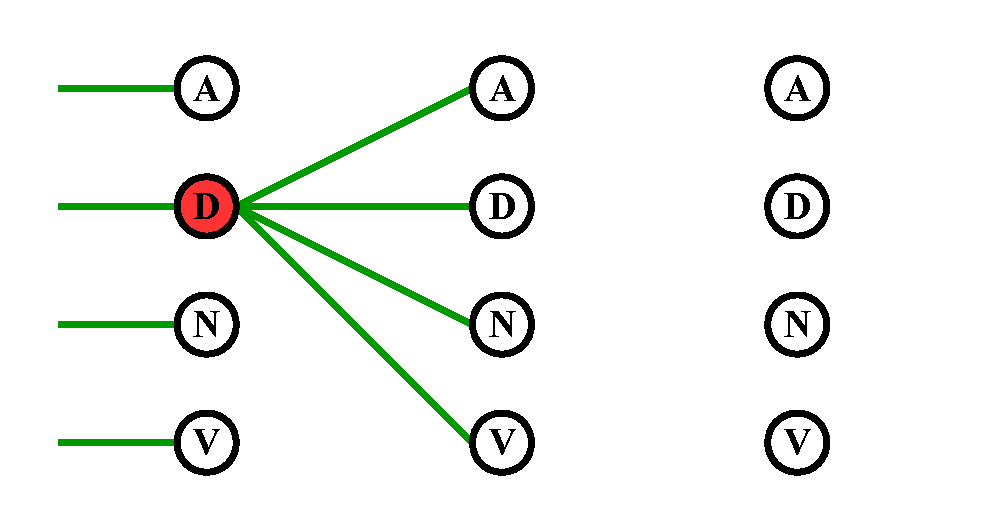
\includegraphics[width=\textwidth]{images/viterbi2}

\vspace{-0.5cm}
\hspace{1.6cm}``The" \hspace{2cm} ``dog" \hspace{2cm} ``ran" 
}
\frame{\frametitle{Viterbi Visualized}
{\bf Viterbi}: Find the highest probability word by word.\\
\hspace{1.55cm} The number of calculations: $(\# words)\paren{\# tags}^{3}$

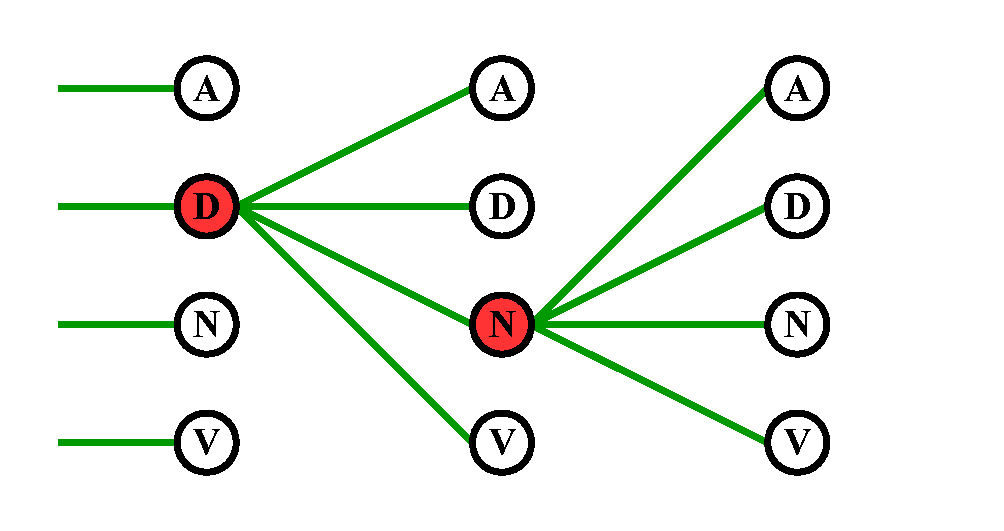
\includegraphics[width=\textwidth]{images/viterbi3}

\vspace{-0.5cm}
\hspace{1.6cm}``The" \hspace{2cm} ``dog" \hspace{2cm} ``ran" 
}
\frame{\frametitle{Viterbi Visualized}
{\bf Viterbi}: Find the highest probability word by word.\\
\hspace{1.55cm} The number of calculations: $(\# words)\paren{\# tags}^{3}$

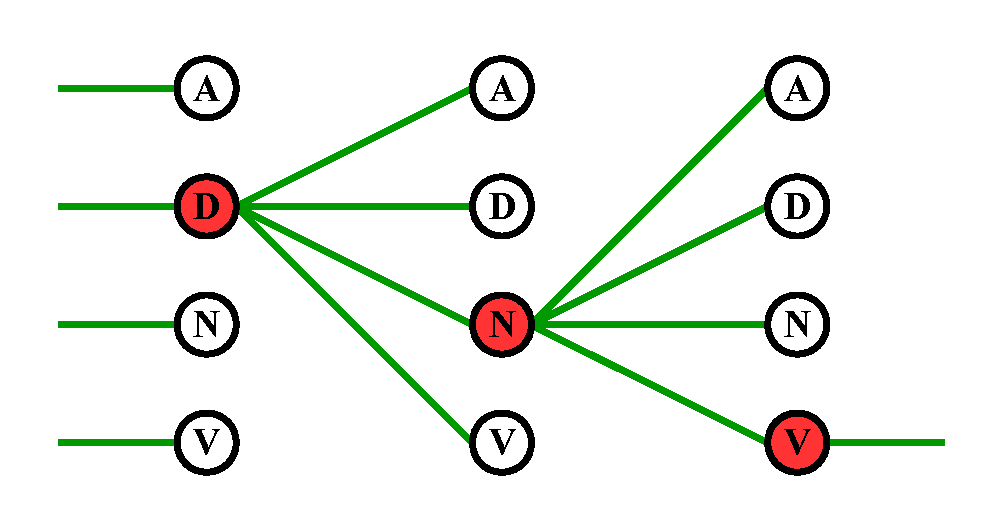
\includegraphics[width=\textwidth]{images/viterbi4}

\vspace{-0.5cm}
\hspace{1.6cm}``The" \hspace{2cm} ``dog" \hspace{2cm} ``ran" 
}



\subsection{References and Resources}
%================================================================================%
%                                    REFERENCES                                  %
%================================================================================%
\frame{\frametitle{References and Resources}
This presentation was created using the following sources.

\begin{itemize}
\item 
  {Columbia University's Coursera Course on Natural Language Processing}.\\
  {\tiny \href{https://www.youtube.com/watch?v=kHvoHUGUitQ&list=PLO9y7hOkmmSGSJA8S3gTigcyNDVJ31LLt}{https://www.youtube.com/playlist?list=PLO9y7hOkmmSGSJA8S3gTigcyNDVJ31LLt}}

\item {Tagging with Hidden Markov Models by Michael Collins}.\\
{\tiny \href{http://www.cs.columbia.edu/~mcollins/courses/nlp2011/notes/hmms.pdf}{http://www.cs.columbia.edu/$\sim$mcollins/courses/nlp2011/notes/hmms.pdf}}

\item {A Well-Commented Examples of a Bigram Model By Katrin Erk}.\\
{\tiny \href{http://www.katrinerk.com/courses/python-worksheets/hidden-markov-models-for-pos-tagging-in-python}{http://www.katrinerk.com/courses/python-worksheets/hidden-markov-models-for-pos-tagging-in-python}}
\end{itemize}

}



\end{document}
